% Figure 4: Three-Layer Tower — Translation Functors from Industry to Kernel
% Industry (SynBN) → Superset (SynLP) → Kernel (promoted projections)
\begin{figure}[t]
\centering
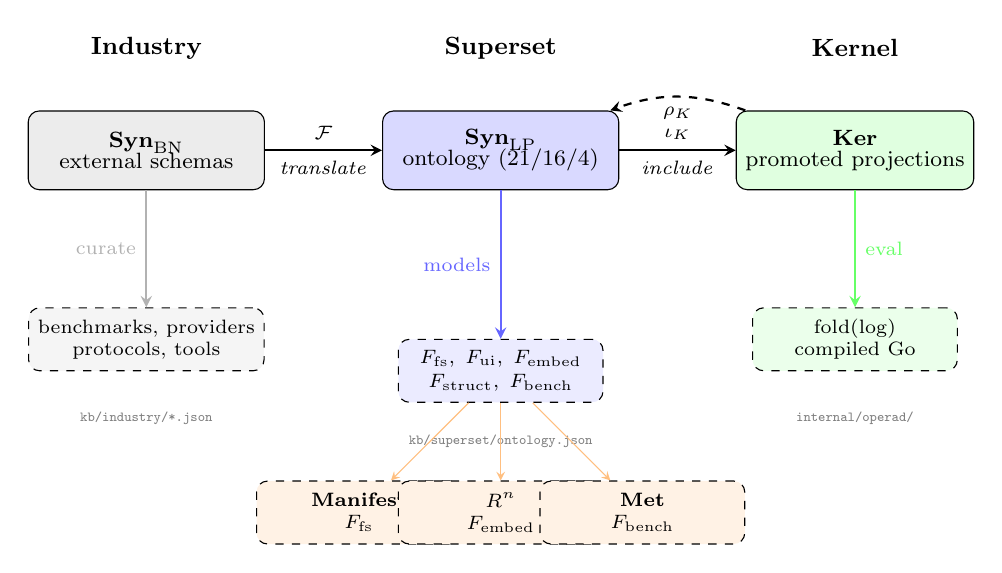
\begin{tikzpicture}[
  box/.style={draw, rounded corners, minimum width=3.0cm, minimum height=1.0cm, align=center, font=\footnotesize},
  sem/.style={draw, rounded corners, dashed, minimum width=2.6cm, minimum height=0.8cm, align=center, font=\scriptsize},
  arrow/.style={->, thick, >=stealth},
  functor/.style={->, thick, >=stealth, font=\small},
  label/.style={font=\scriptsize},
  col/.style={font=\small\bfseries}
]

% Column headers
\node[col] at (-4.5, 4.5) {Industry};
\node[col] at (0, 4.5) {Superset};
\node[col] at (4.5, 4.5) {Kernel};

% Top row: Syntax categories
\node[box, fill=gray!15] (ind) at (-4.5, 3.2) {$\mathbf{Syn}_{\mathrm{BN}}$\\[-2pt] external schemas};
\node[box, fill=blue!15] (sup) at (0, 3.2) {$\mathbf{Syn}_{\mathrm{LP}}$\\[-2pt] ontology (21/16/4)};
\node[box, fill=green!12] (ker) at (4.5, 3.2) {$\mathbf{Ker}$\\[-2pt] promoted projections};

% Horizontal functor arrows (translation)
\draw[functor] (ind) -- node[above, label] {$\mathcal{F}$} node[below, label] {\textit{translate}} (sup);
\draw[functor] (sup) -- node[above, label] {$\iota_K$} node[below, label] {\textit{include}} (ker);

% Adjoint arrow (restrict) — dashed, below
\draw[functor, dashed, bend right=20] (ker) to node[below, label] {$\rho_K$} node[above, label] {} (sup);

% Bottom row: Semantic models (functor images)
\node[sem, fill=gray!8] (sem-ind) at (-4.5, 0.8) {benchmarks, providers\\protocols, tools};
\node[sem, fill=blue!8] (sem-sup) at (0, 0.4) {$F_{\mathrm{fs}},\; F_{\mathrm{ui}},\; F_{\mathrm{embed}}$\\[1pt] $F_{\mathrm{struct}},\; F_{\mathrm{bench}}$};
\node[sem, fill=green!8] (sem-ker) at (4.5, 0.8) {$\mathrm{fold}(\mathrm{log})$\\compiled Go};

% Vertical functor arrows (syntax → semantics)
\draw[arrow, gray!60] (ind) -- node[left, label] {curate} (sem-ind);
\draw[arrow, blue!60] (sup) -- node[left, label] {models} (sem-sup);
\draw[arrow, green!60] (ker) -- node[right, label] {eval} (sem-ker);

% File path annotations (grounding in codebase)
\node[font=\tiny\ttfamily, text=gray] at (-4.5, -0.2) {kb/industry/*.json};
\node[font=\tiny\ttfamily, text=gray] at (0, -0.5) {kb/superset/ontology.json};
\node[font=\tiny\ttfamily, text=gray] at (4.5, -0.2) {internal/operad/};

% Target categories fan-out from superset
\node[sem, fill=orange!10] (t1) at (-1.8, -1.4) {\textbf{Manifest}\\$F_{\mathrm{fs}}$};
\node[sem, fill=orange!10] (t2) at (0, -1.4) {$\mathbb{R}^n$\\$F_{\mathrm{embed}}$};
\node[sem, fill=orange!10] (t3) at (1.8, -1.4) {\textbf{Met}\\$F_{\mathrm{bench}}$};

\draw[arrow, orange!50, thin] (sem-sup) -- (t1);
\draw[arrow, orange!50, thin] (sem-sup) -- (t2);
\draw[arrow, orange!50, thin] (sem-sup) -- (t3);

\end{tikzpicture}
\caption{The three-layer tower. Industry data enters via the translation functor
$\mathcal{F}\colon \mathbf{Syn}_{\mathrm{BN}} \to \mathbf{Syn}_{\mathrm{LP}}$.
The superset ontology serves as the free category whose models (FUN01--FUN05) are
structure-preserving functors to target categories. Stable patterns are promoted
into the kernel via $\iota_K$; the kernel exposes its structure back to the graph
via $\rho_K$ (the adjoint restriction). File paths ground each layer in the
codebase.}
\label{fig:tower}
\end{figure}
